% Section with miscellaneous contents


\section{Sonstiges (Floats, Zitationen, etc.)}


\subsection{Unterabschnitt mit Zitationen}
Dies ist eine Zitation~\cite{D0.ConfNote.5607} und dies eine weitere~\cite{PhysRevLett.100.192004}. Und mehrere Zitationen auf einmal~\cite{PhysRevLett.74.2632, PhysRevLett.100.192004, PhysRevLett.74.2626}.
\blindtext


\subsection{Unterabschnitt mit Figures}
\blindtext
%
\begin{figure*}[t]
  \centering
  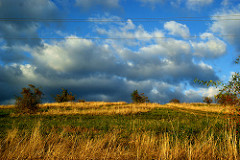
\includegraphics[width=0.49\textwidth]{example.jpg}
  \caption{\blindtext}
  \label{fig:1}
\end{figure*}
%
\blindtext
%
\begin{figure}[t]
  \centering
  \subcaptionbox{\label{fig:3.1}Erste Bildunterschrift.}{%
    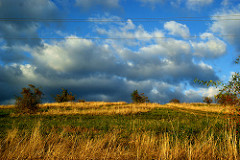
\includegraphics[width=0.24\textwidth]{example.jpg}%
  }~
  \subcaptionbox{\label{fig:3.2}Zweite Bildunterschrift.}{%
    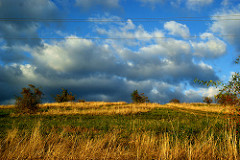
\includegraphics[width=0.24\textwidth]{example.jpg}
  }
  \caption{Bildunterschrift der gesamten Figure mit Referenzen auf~\cref{fig:3.1} and~\cref{fig:3.2}.}
  \label{fig:3}
\end{figure}
%
\blindtext


\subsection{Unterabschnitt mit Referenzen}
Dies hier ist eine Referenz auf \cref{fig:1}. Und dies eine andere Referenz auf \cref{eq:1}, welche sich in \cref{sec:maths-incl-subeq} befindet. Und das hier ist eine Referenz auf \cref{fig:3.1}, welche Teil von \cref{fig:3} ist. \blindtext


\subsection{Unterabschnitt mit Tabelle}
\blindtext

\begin{table}[tb]
  \centering
  \caption{Dies ist die Tabellenbeschreibung.}
  \begin{tabular}{l l l l l l l}
    \toprule
    OrderDate & Region & Rep & Item & Units & Cost & Total \\
    \midrule
    1/6/2014 & East & Jones & Pencil & 95 & 1.99 & 189.05 \\
    1/23/2014 & Central & Kivell & Binder & 50 & 19.99 & 999.50 \\
    2/9/2014 & Central & Jardine & Pencil & 36 & 4.99 & 179.64 \\
    2/26/2014 & Central & Gill & Pen & 27 & 19.99 & 539.73 \\
    3/15/2014 & West & Sorvino & Pencil & 56 & 2.99 & 167.44 \\
    4/1/2014 & East & Jones & Binder & 60 & 4.99 & 299.40 \\
    4/18/2014 & Central & Andrews & Pencil & 75 & 1.99 & 149.25 \\
    5/5/2014 & Central & Jardine & Pencil & 90 & 4.99 & 449.10 \\
    \bottomrule
  \end{tabular}
  \label{tab:1}
\end{table}
%
\blindtext


% End of file
